\documentclass[a4paper,11pt]{article}
\setcounter{secnumdepth}{-1}
\usepackage[spanish]{babel}
\usepackage{graphicx}
\usepackage[ansinew]{inputenc}
\usepackage[utf8]{inputenx}
\usepackage{listings}
\usepackage{xcolor}
\usepackage{hyperref}
\hypersetup{
    colorlinks=true, %set true if you want colored links
    linktoc=all,     %set to all if you want both sections and subsections linked
    linkcolor=black,  %choose some color if you want links to stand out
}

\lstdefinestyle{neo4j}{
breaklines,
backgroundcolor=\color{lightgray},
keywordstyle=*\color{blue},
otherkeywords = {MATCH, LIMIT, WITH, ORDER, BY, WHERE},
morekeywords = [2]{MATCH, LIMIT, WITH, ORDER, BY, WHERE},
frame=single, 
language={[77]Fortran}, 
columns=fullflexible}


\title{\textbf{Trabajo Práctico Aéreos} \\[1cm] 
\includegraphics[scale=1]{./imagenes/fiuba.png}}

\author{	Francisco Hermani, \textit{Padrón Nro. 98223}                     \\
            \texttt{ franhermani@gmail.com }                                              \\[2.5ex]
            Cotarelo Rodrigo, \textit{Padrón Nro. 98577}                     \\
            \texttt{ cotarelorodrigo@gmail.com }                                              \\[2.5ex]
			Agostina Vázquez, \textit{Padrón Nro. 99689}                    
\\
            \texttt{ agostinavazquezisla@gmail.com }                                              \\[2.5ex]
            \normalsize{1er. Cuatrimestre de 2019}                                      \\
            \normalsize{95.02 Base de Datos}  \\
            \normalsize{Facultad de Ingeniería, Universidad de Buenos Aires}            \\
       }
\date{26/06/2019}


\begin{document}

\maketitle
\thispagestyle{empty}   % quita el número en la primer página
\newpage
{\sffamily\tableofcontents}
\newpage
\section{Parser de los archivos HTML provistos por la cátedra}
Este punto fue implementado exclusivamente en el notebook html scrapper, con el objetivo principal de interpretar y parsear los archivos HTML que nos proporcionó la cátedra para obtener una información preliminar de los vuelos.Así, logramos generar una serie de archivos pkl con los siguientes atributos de cada vuelo: aerolínea, horario de salida y de llegada, terminal de salida y de llegada, puerta de salida y de llegada, origen y destino. En puntos posteriores se verá que no todos los atributos nos resultaron de gran valor, razón por la cual algunos fueron dejados de lado.

\section{Concatenación de los archivos pkl}
Para facilitar posteriores operaciones, decidimos concatenar los archivos pkl obtenidos. Al mismo tiempo, analizamos más detenidamente los datos y les aplicamos un formato más acorde.
Esto fue realizado en el notebook pkl generator.

\section{Análisis de los datos obtenidos}
Como paso intermedio, tal vez no tan relacionado con la consigna principal del trabajo, realizamos una serie de análisis estadísticos de la información que teníamos hasta el momento.
De esta forma, en el notebook analysis obtuvimos métricas como:
\begin{itemize}
\item Top 10 de aerolíneas con mayor cantidad de vuelos
\begin{center}
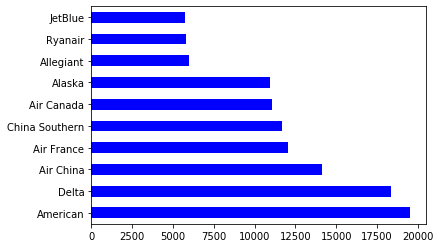
\includegraphics[scale=0.60]{./imagenes/aerolineas_top10.png}
\end{center}
\newpage
\item Días y horarios con mayor cantidad de vuelos
\begin{center}
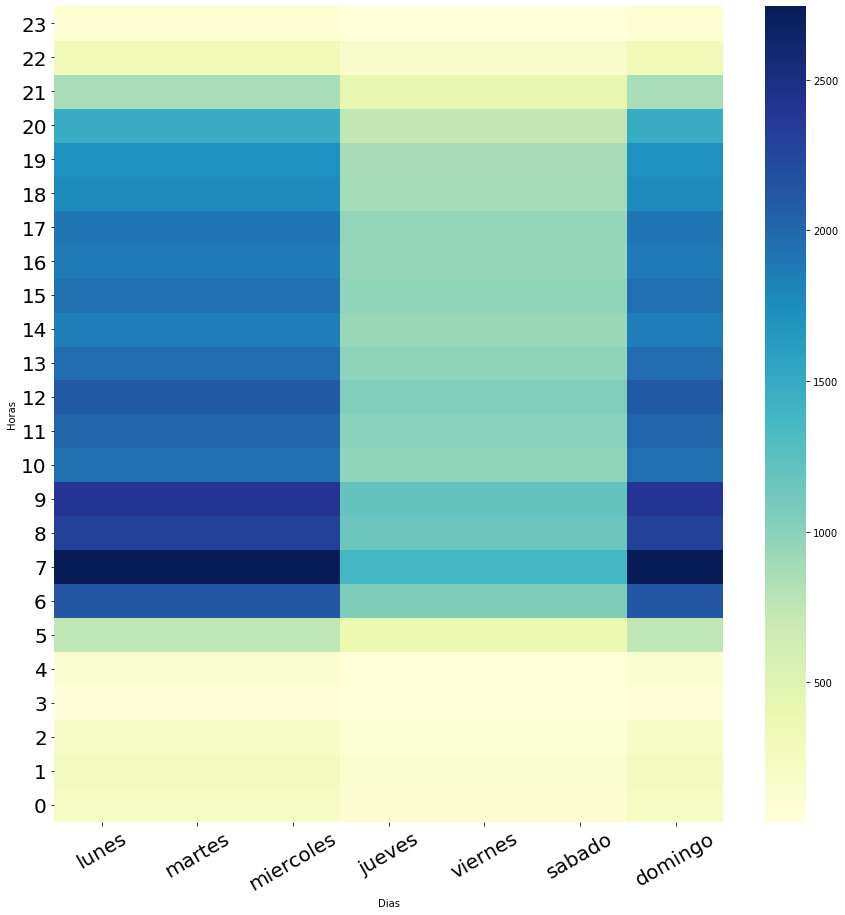
\includegraphics[scale=0.35]{./imagenes/heatmap.png}
\end{center}
\item Destinos más frecuentes
\begin{center}

\includegraphics[scale=0.35]{./imagenes/wordcloud.png}
\end{center}
\end{itemize}
\newpage
\section{Generación de la información completa de los vuelos}
Retomando el flujo original del trabajo, apuntamos a generar el archivo definitivo de vuelos (primera versión al menos), con información consistente para utilizar en el Neo4j y suficiente para las consultas propuestas.
Para ello, hicimos uso del notebook csv generator, en donde transformamos el archivo pkl en un formato csv para luego importarlo en el Neo4j.
Aquí es donde aplicamos la mayor limpieza de datos y cálculo de ciertos atributos. Asimismo, investigamos bastante sobre los tipos de datos aceptados por el Neo4j, por lo cual realizamos ciertas operaciones de formato en base a esto. Se destacan como puntos más importantes:
\begin{itemize}
\item Eliminación de espacios innecesarios provenientes de los HTML
\item Conversión de fechas y horarios en un único timestamp
\item Cálculo de la duración de cada vuelo
\item Cálculo del precio de cada vuelo (proporcional a la distancia recorrida)
\item Generación aleatoria de asientos disponibles de cada vuelo
\item Modificaciones varias y eliminación de columnas innecesarias
\end{itemize}
Cabe aclarar que este punto no resultó tan trivial como parece.
En principio, como no teníamos el costo de los vuelos, intentamos hacer uso de la API de Skyscanner. Para ello, investigamos sobre los endpoints que proveía y no logramos dar con el adecuado. Por ejemplo, uno carecía del costo del vuelo (nos colocaba en la misma situación que antes) y otro carecía del horario de llegada (lo cual era aún más limitante para la consigna del trabajo).
Ante este dead-end, apostamos por obtener las distancias entre los aeropuertos mediante una función matemática y asignar un precio a cada vuelo proporcional a la distancia recorrida. Esto lo logramos gracias al archivo aeropuertos.csv proporcionado por la cátedra, que contenía las coordenadas de cada aeropuerto.
\newpage
\section{Lecturas sobre bases de datos orientadas a grafos y el lenguaje Cypher}
Esta etapa fue principalmente de investigación sobre el lenguaje que utilizaríamos para las consultas. Junto con esto, tuvimos que fortalecer nuestros conocimientos teóricos sobre las bases de datos orientadas a grafos.
Para ello, acudimos a los manuales provistos por la cátedra (Graph Databases y Learning Cypher) y a los tutoriales interactivos y manual oficial del Neo4j.

\section{Instalación del Neo4j}
A priori, una persona ajena al grupo podría creer que esta etapa fue la más trivial. Nada más alejado de eso.
Instalamos distintas versiones del Neo4j Desktop en distintos sistemas operativos (Linux y Windows) y siempre nos encontramos con algún inconveniente. Por ejemplo, algunas versiones nos mostraban una pantalla en blanco al iniciar el programa, sin opción alguna de avanzar. Otras no nos permitían pasar al modo online para descargar plugins.
Para poder avanzar, decidimos hacer uso de los sandbox que proporciona Neo4j, una especie de versión online con fecha de expiración. En este entorno fue en donde realizamos la mayor parte de las pruebas.

\section{Primer approach para resolver las consultas}
Nuestra primera interpretación de las consultas nos llevó a pensar que debíamos hacer uso de algún algoritmo de camino mínimo en grafos. Fue entonces que investigamos al respecto y nos encontramos con las librerías APOC y ALGO, las cuales proporcionan un conjunto de algoritmos de grafos que, aparentemente, cumplían con nuestros requisitos.
El primer problema con el que nos encontramos fue que, como se mencionó antes, nuestro Neo4j Desktop no podía cambiar a modo online, por lo cual no podíamos instalar los plugins necesarios para hacer uso de dichas librerías.
Para sortear este inconveniente utilizamos los sandbox. A pesar de que los plugins ya estaban instalados en este entorno, nos encontramos con un error en la consulta que desarrollamos que no supimos resolver.
Se detalla a continuación la consulta propuesta en su momento:
\newpage
\begin{lstlisting}[style=neo4j]
WITH 'Indiana' AS origen, 'Zanzibar' AS destino
MATCH (inicio: Ciudad { nombre: origen }), (fin: Ciudad { nombre: destino })
CALL algo.shortestPath(inicio, fin, 'hora_llegada',{ relationshipQuery:
'MATCH (a: Ciudad {nombre: origen})-[v1:VUELO]-()-[v2:VUELO]->(b: Ciudad {nombre: destino})
WHERE localdatetime(v1.hora_llegada) < localdatetime(v2.hora_salida)', graph:'cypher'})
YIELD nodeCount, totalCost, loadMillis, evalMillis, writeMillis
RETURN 	nodeCount AS cant_ciudades,
		totalCost AS duracion_total,
		loadMillis AS tiempo_carga,
		evalMillis AS tiempo_algoritmo,
		writeMillis AS tiempo_escritura
\end{lstlisting}
Como se puede ver, hicimos uso de la librería ALGO, en particular de la función shortestPath. A su vez, para resolver las restricciones propias del problema, aplicamos subconsultas sobre las relaciones resultantes del camino obtenido.
Sin embargo, nunca lo pudimos hacer funcionar, obteniendo siempre el siguiente error:
\begin{lstlisting}[style=neo4j]
Neo.ClientError.Procedure.ProcedureCallFailed: Failed to invoke 
procedure `algo.shortestPath`:
Caused by: java.lang.NullPointerException
\end{lstlisting}

\section{Segundo approach para resolver las consultas}
En el mismo momento que decidimos dejar de lado el uso de librerías por los reiterados inconvenientes técnicos, nos dimos cuenta que nuestra primera interpretación del problema fue errónea: estábamos apuntando a minimizar la duración total de los vuelos, cuando en realidad el objetivo era encontrar el camino cuyo último vuelo tenga la menor hora de llegada.
Una vez que entendimos esto, investigamos aún más sobre el lenguaje Cypher y las posibilidades que ofrecía, hasta dar con la solución a ambas consultas.
Para comprobar su correcto funcionamiento, implementamos pequeños datasets con restricciones apropiadas y distintas variantes de caminos.

\newpage
\section{Regeneración del set de datos}
En base a lo charlado en clase, volvimos a generar el set de datos, reduciendo la cantidad de vuelos (había muchos similares entre un mismo origen y destino pero con una diferencia mínima de horarios) e instanciándolos durante 10 días a partir de la fecha actual de ejecución del script.

\section{Carga del set de datos en el Neo4j y creación de la base de datos}
Para este punto, utilizamos el comando LOAD CSV en conjunto con el MERGE, para lograr importar los datos y crear la base de datos a partir de ellos en una misma instrucción.
La carga del archivo tardó aproximadamente siete minutos y medio con el primer set de datos y poco más de dos minutos con el set final.

\section{Ejecución de las consultas con los datos reales}
Finalmente, ejecutamos las consultas en el lenguaje Cypher. Los resultados obtenidos se detallarán en la sección Consultas.

\newpage
\section*{Comandos utilizados}
\addcontentsline{toc}{section}{Comandos utilizados}
A continuación, se listan una serie de comandos que utilizamos reiteradas veces a lo largo del trabajo:
\bigbreak
\noindent
\underline{Limpiar la base de datos completa}\\
\noindent
\\
MATCH (n) DETACH DELETE n
\bigbreak
\noindent
\underline{Mostrar la base de datos completa}\\
\noindent
\\
MATCH (n) RETURN n
\bigbreak
\noindent
\underline{Importar archivos muy grandes}\\
\noindent
\\
USING PERIODIC COMMIT
\bigbreak
\noindent
\underline{Importar CSV al Neo4j y crear nodos y relaciones}\\

Previamente, debe colocarse el archivo csv en la carpeta import del Neo4j.
\begin{lstlisting}[style=neo4j]
LOAD CSV WITH HEADERS FROM "file:///info_vuelos.csv" AS vuelos
MERGE (a:Ciudad { nombre: vuelos.origen })
MERGE (b:Ciudad { nombre: vuelos.destino })
MERGE (a)-[:VUELO
	{ aerolinea: vuelos.aerolinea,
	hora_salida: vuelos.hora_salida,
	hora_llegada: vuelos.hora_llegada,
	duracion: vuelos.duracion,
	precio: vuelos.precio,
	asientos: vuelos.asientos_disponibles }]->(b)
\end{lstlisting}

\newpage
\section*{Consultas}
\addcontentsline{toc}{section}{Consultas}
ACLARACIÓN: las consultas que propuso la cátedra fueron proporcionadas con variables cuyos valores, en algunos casos, no pudimos respetar. En particular, se dieron los siguientes casos:
\begin{itemize}
\item Ninguna de las ciudades mencionadas (Indiana, Zanzibar y Gibraltar) están presentes en nuestro set de datos final.
\item Ningún vuelo tiene un precio menor a \$4000. De hecho, nuestros precios están en USD.
\end{itemize}
    
Por ello, decidimos realizar las consultas con otros valores que, igualmente, son parametrizables por el usuario.
A su vez, limitamos la cantidad de vuelos a un valor razonable, ya que de lo contrario obteníamos error de memoria.
Para ello, la instrucción [vuelos:VUELO*] se reemplazó por [vuelos:VUELO*1..N], siendo N la cantidad límite de vuelos en el camino.

Garfield quiere irse de vacaciones a la paradisíaca isla de Zanzíbar en el Océano Índico.
A) Encuentre un itinerario de modo que Garfield llegue lo antes posible a Zanzibar saliendo desde su hogar en “Indiana, IL” mañana.
\begin{lstlisting}[style=neo4j]
WITH
'Indiana' AS origen,
'Zanzibar' AS destino,
1 AS cant_pasajeros
MATCH path=(start: Ciudad {nombre: origen})-[vuelos:VUELO*]->(end:
Ciudad {nombre: destino})
WITH path, LAST(vuelos) as ultimo_vuelo, NODES(path) as ciudades
WHERE ALL (vuelo in vuelos WHERE toInt(vuelo.asientos) >=
cant_pasajeros)
AND ALL (i in Range(0, length(vuelos) - 2) WHERE 
(vuelos[i]).hora_llegada < (vuelos[i+1]).hora_salida)
RETURN path, EXTRACT (ciudad in ciudades | ciudad.nombre) as ciudades
ORDER BY ultimo_vuelo.hora_llegada ASC
LIMIT 1
\end{lstlisting}

B) Encuentre un segundo itinerario que resuelva los siguientes problemas:
- Asegúrese de que todos los vuelos cuenten con dos lugares disponibles, ya que Garfield quiere llevar también a Odie.
- Asegúrese de que el costo no supere el presupuesto de Garfield, que es de 2000 pesos por individuo (4000 pesos en total).
- Asegúrese de que el vuelo encontrado no pase por Gibraltar, ya que su pista de aterrizaje es una de las más peligrosas del mundo, y Garfield definitivamente no quiere pasar por allí.
\newpage
\begin{lstlisting}[style=neo4j]
WITH
'Indiana' AS origen,
'Zanzibar' AS destino,
'Gibraltar' AS peligro,
2 AS cant_pasajeros,
4000 AS precio_max
MATCH path=(start: Ciudad {nombre: origen})-
[vuelos:VUELO*]->(end: Ciudad {nombre: destino})
WITH path, REDUCE(weight = 0, vuelo in vuelos | weight +
toInt(vuelo.precio) * cant_pasajeros) as precio_total, LAST(vuelos) as
ultimo_vuelo, NODES(path) as ciudades
WHERE precio_total <= precio_max
AND ALL (vuelo in vuelos WHERE toInt(vuelo.asientos) >=
cant_pasajeros)
AND ALL (i in Range(0, length(vuelos) - 2) WHERE
(vuelos[i]).hora_llegada < (vuelos[i+1]).hora_salida)
AND ALL (ciudad in ciudades WHERE ciudad.nombre <> peligro)
RETURN path, EXTRACT (ciudad in ciudades | ciudad.nombre) as ciudades,
precio_total
ORDER BY ultimo_vuelo.hora_llegada ASC
LIMIT 1
\end{lstlisting}

\newpage
\section*{Resultados obtenidos}
\addcontentsline{toc}{section}{Resultados obtenidos}
Como se mencionó antes, las consultas las ejecutamos con valores distintos a los propuestos por la cátedra.
A continuación, se detallan los resultados obtenidos:
\linebreak
\subsection*{Consulta A}
\subsubsection*{Ejecucion 1}
\noindent
\underline{Parámetros}
\begin{itemize}
\item Origen: Barcelona
\item Destino: Miami
\item Límite de vuelos: 3
\end{itemize}
\underline{Resultados}
\begin{itemize}
\item Camino encontrado: Barcelona $\rightarrow$ Miami
\item Tiempo de ejecución: 1 hora y 56 minutos.
\end{itemize}
\begin{center}
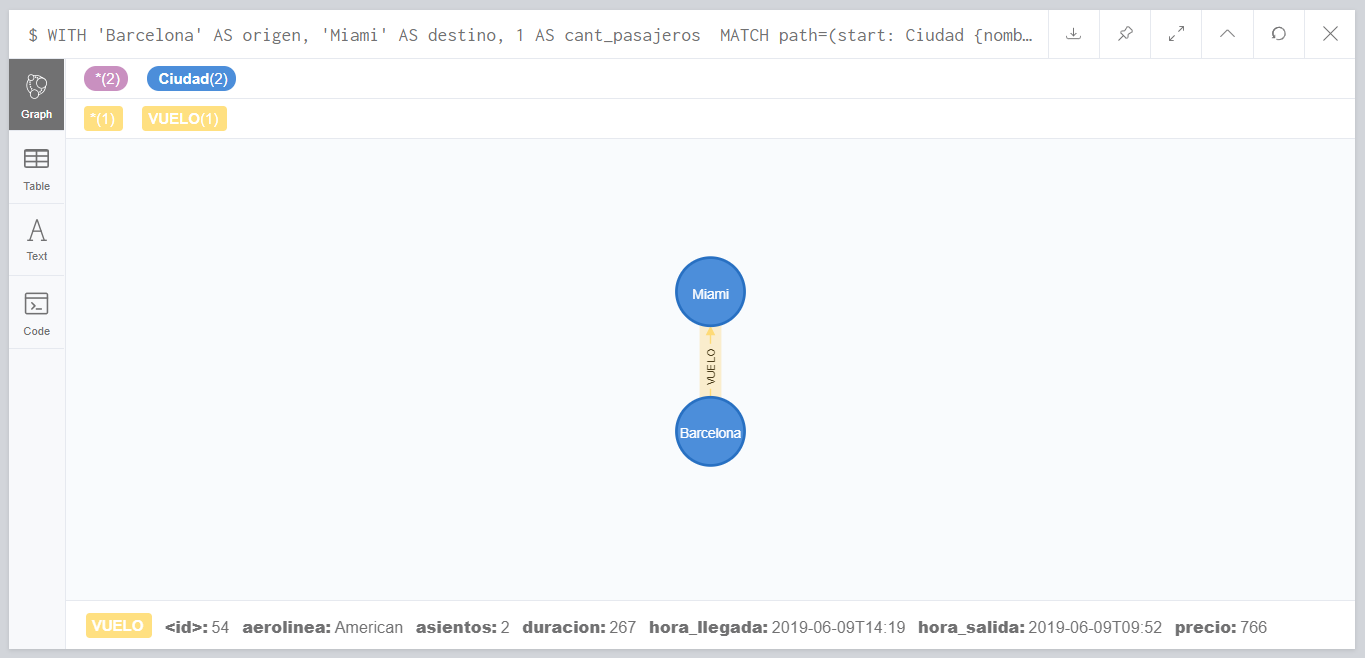
\includegraphics[scale=0.40]{./imagenes/consultaA.png}
\end{center}
\newpage
\subsubsection*{Ejecucion 2}
\noindent
\underline{Parámetros}
\begin{itemize}
\item Origen: Madrid
\item Destino: Hong Kong
\item Límite de vuelos: 3
\end{itemize}
\underline{Resultados}
\begin{itemize}
\item Camino encontrado: Madrid $\rightarrow$ Helsinki $\rightarrow$ Hong Kong
\item Tiempo de ejecución: 28 minutos.
\end{itemize}
\begin{center}
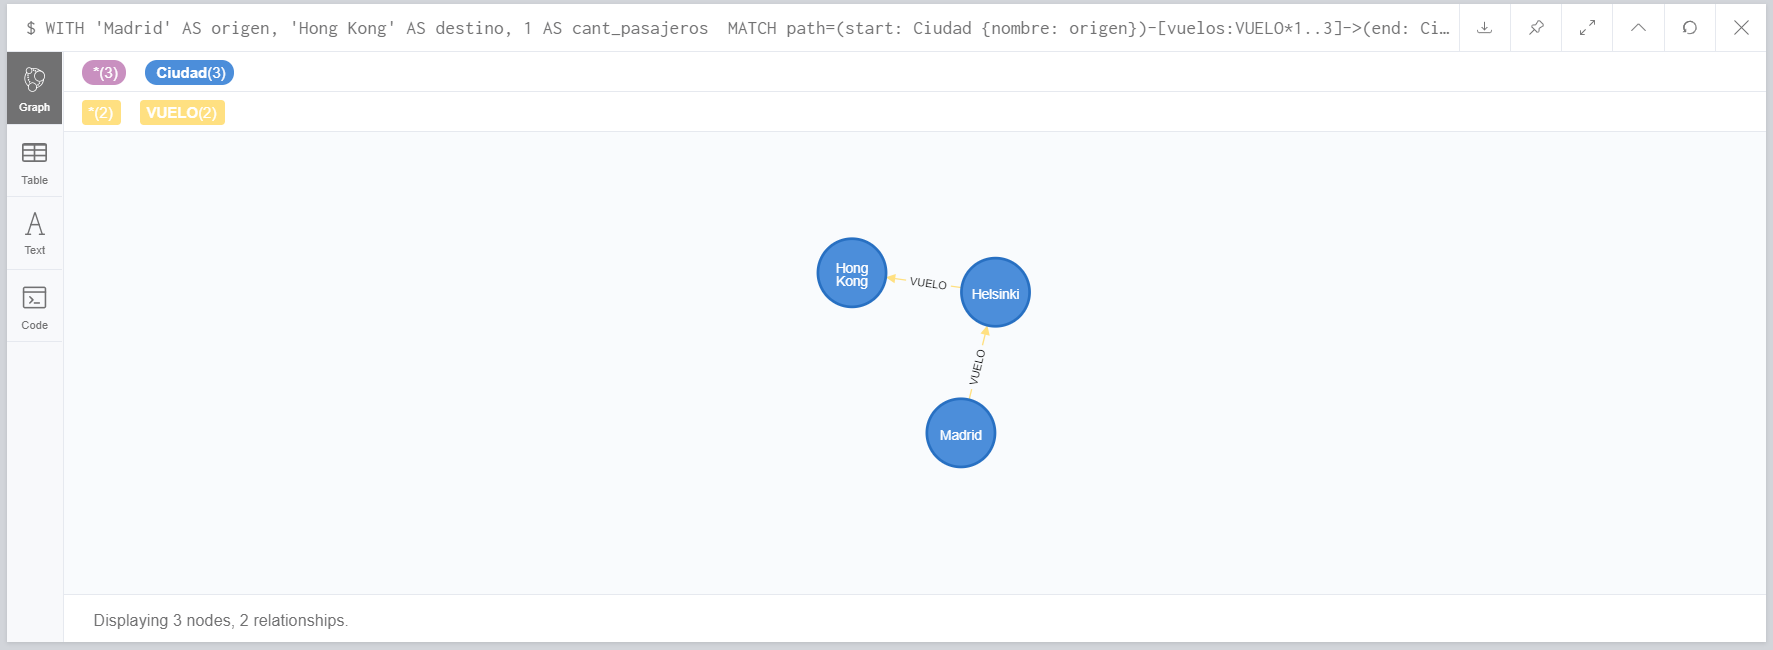
\includegraphics[scale=0.40]{./imagenes/consultaA-ejec2.png}
\end{center}
\newpage
\subsubsection*{Ejecucion 3}
\noindent
\underline{Parámetros}
\begin{itemize}
\item Origen: Budapest
\item Destino: Arequipa
\item Límite de vuelos: 3
\end{itemize}
\underline{Resultados}
\begin{itemize}
\item Camino encontrado: Budapest $\rightarrow$ Madrid $\rightarrow$ Lima $\rightarrow$ Arequipa
\item Tiempo de ejecución: 50 segundos
\end{itemize}
\begin{center}
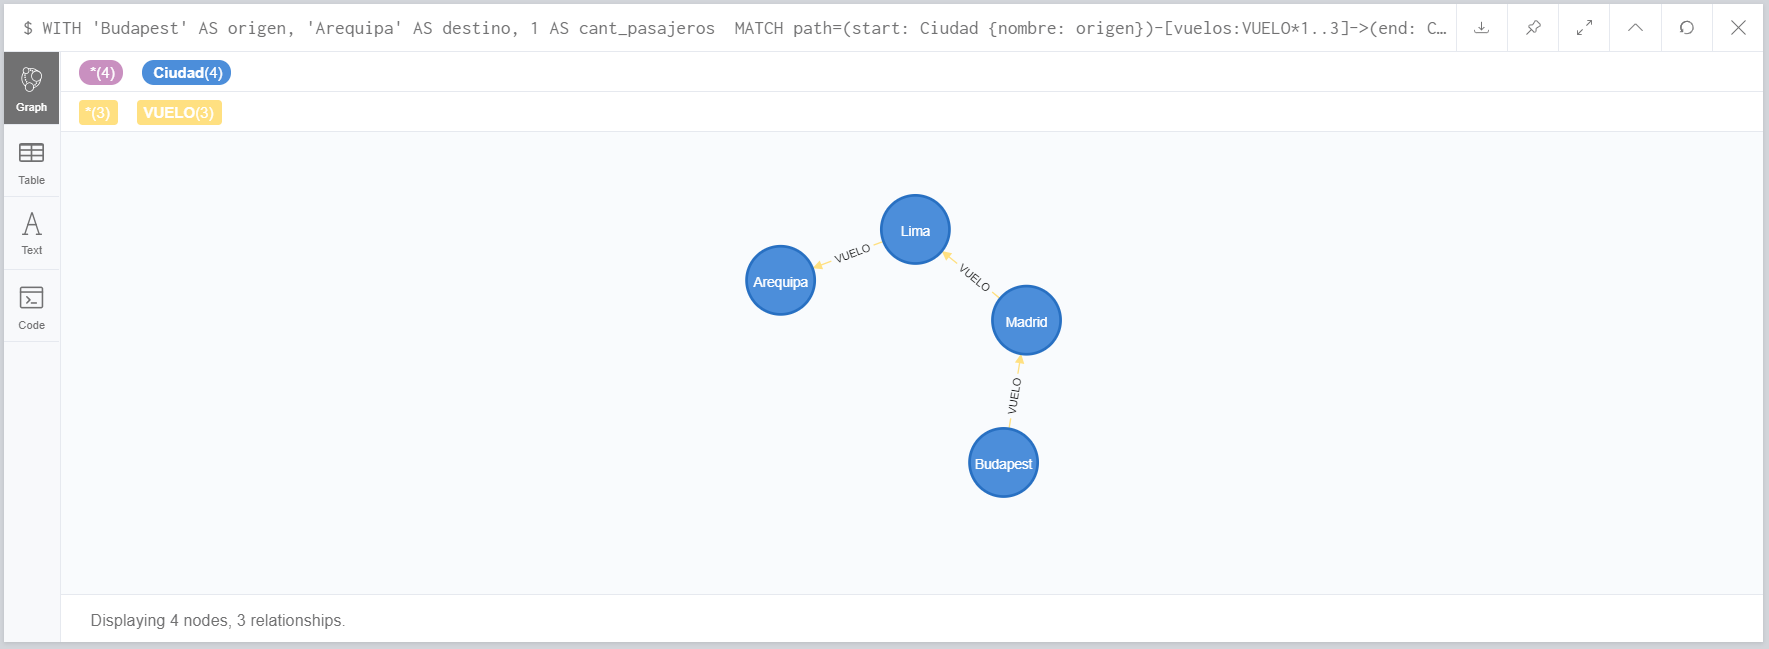
\includegraphics[scale=0.40]{./imagenes/consultaA-ejec3.png}
\end{center}
\newpage
\subsection*{Consulta B}
\subsubsection*{Ejecucion 1}
\noindent
\underline{Parámetros}
\begin{itemize}
\item Origen: Liverpool
\item Destino: Lima
\item Peligro: Londonderry
\item Precio máximo: 6000 USD
\item Límite de vuelos: 4
\end{itemize}
\underline{Resultados}
\begin{itemize}
\item Camino encontrado: -
\item Tiempo de ejecución: 8 horas y frenamos la ejecución.
\end{itemize}
Ante la larga ejecución del algoritmo, decidimos frenarla e intentar nuevamente, pero con un límite de vuelos igual a 3.
El camino encontrado fue Liverpool $\rightarrow$ Fuerteventura $\rightarrow$ Madrid $\rightarrow$ Lima, con un tiempo de ejecución total de 12 minutos.\\
\begin{center}
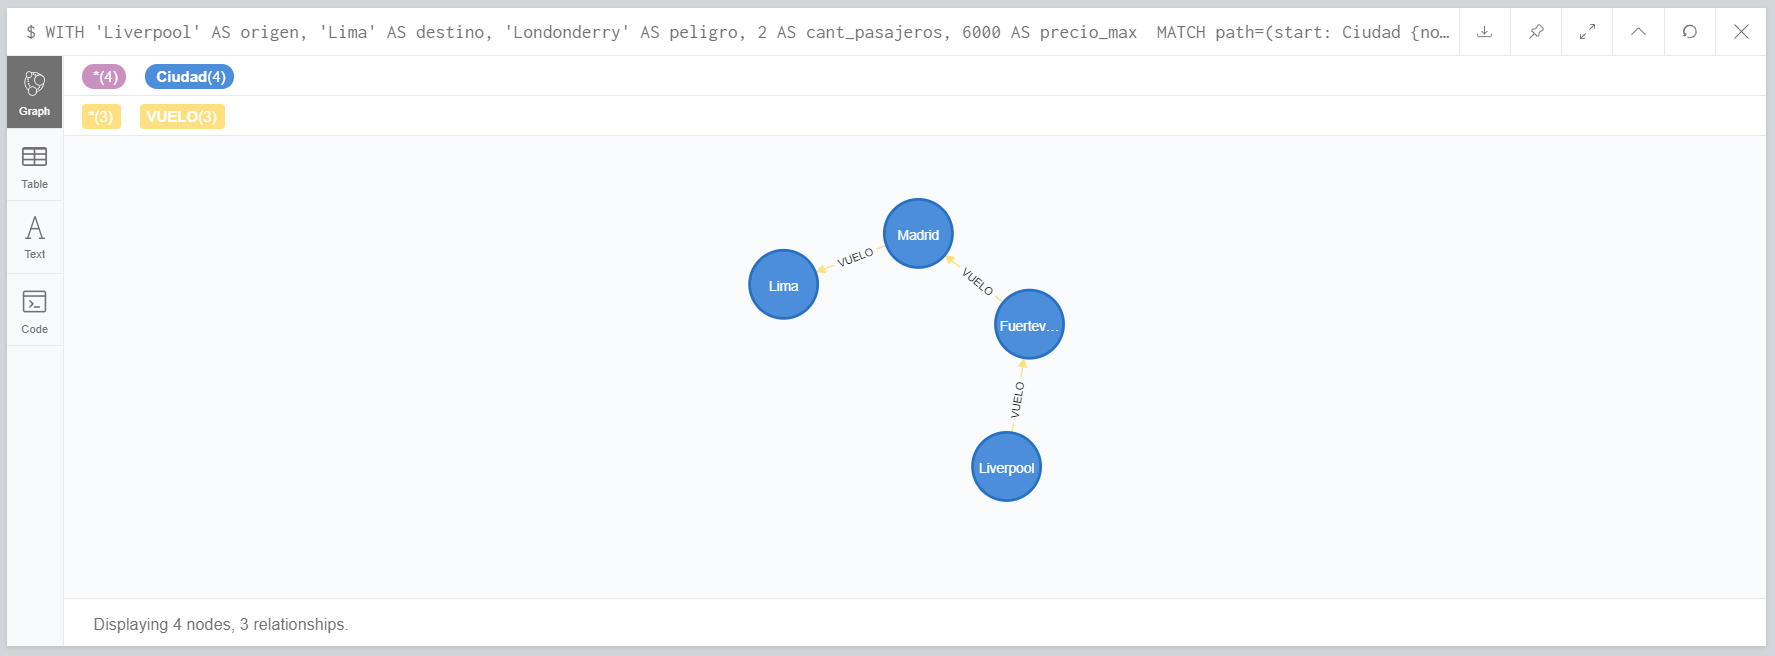
\includegraphics[scale=0.40]{./imagenes/consultaB-ejec1.png}
\end{center}
\newpage
\subsubsection*{Ejecucion 2}
\noindent
\underline{Parámetros}
\begin{itemize}
\item Origen: Lima
\item Destino: Birmingham
\item Peligro: Atlanta
\item Precio máximo: 4000 USD
\item Límite de vuelos: 3
\end{itemize}
\underline{Resultados}
\begin{itemize}
\item Camino encontrado: Lima $\rightarrow$ Miami $\rightarrow$ Birmingham
\item Tiempo de ejecución: 15 minutos
\end{itemize}
\begin{center}
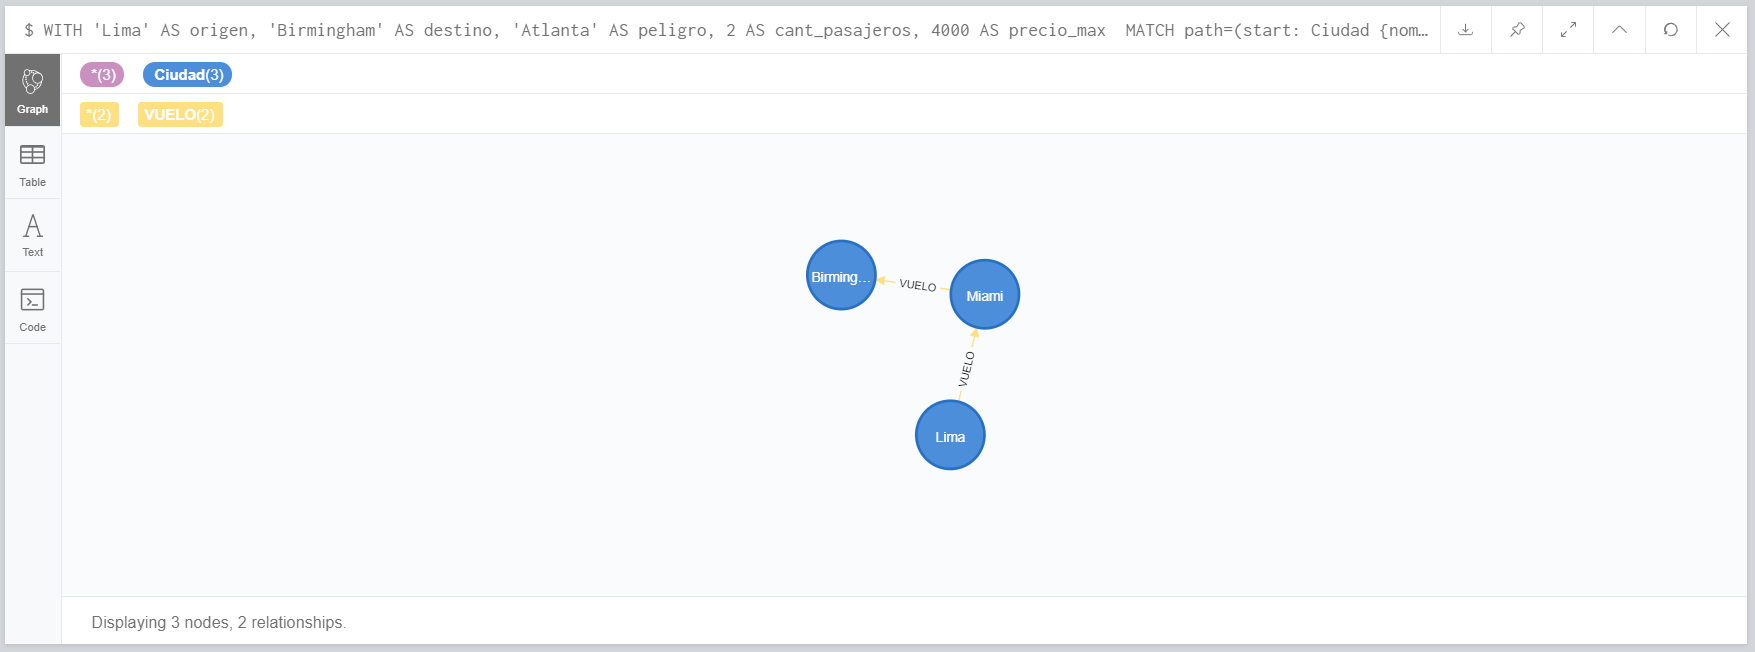
\includegraphics[scale=0.40]{./imagenes/consultaB-ejec2.png}
\end{center}
\newpage
\subsubsection*{Ejecucion 3}
\noindent
\underline{Parámetros}
\begin{itemize}
\item Origen: Madrid
\item Destino: Hong Kong
\item Peligro: Helsinki
\item Precio máximo: 7000 USD
\item Límite de vuelos: 3
\end{itemize}
\underline{Resultados}
\begin{itemize}
\item Camino encontrado: Madrid $\rightarrow$ Atlanta $\rightarrow$ Melbourne $\rightarrow$ Hong Kong
\item Tiempo de ejecución: 29 minutos
\end{itemize}
\begin{center}
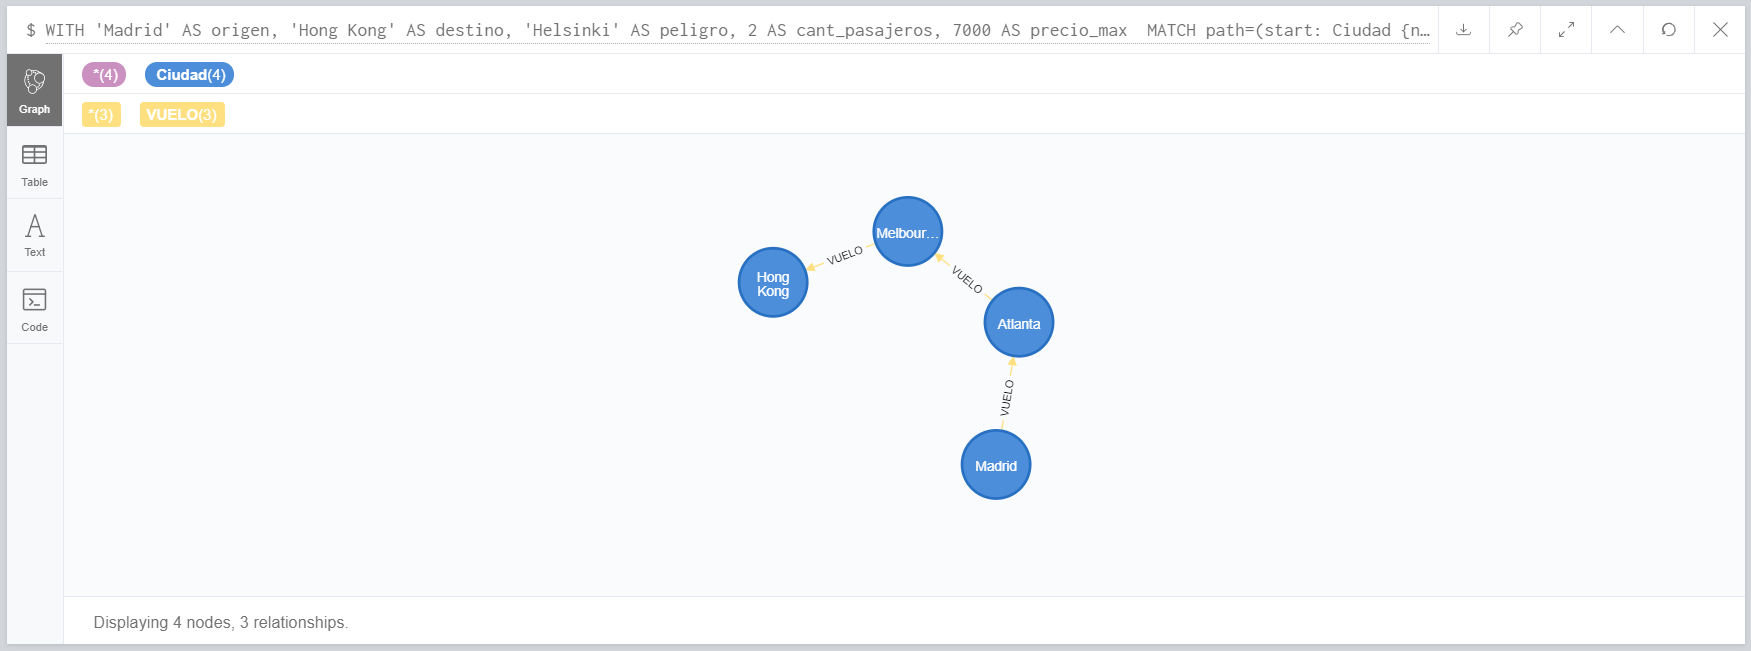
\includegraphics[scale=0.40]{./imagenes/consultaB-ejec3.png}
\end{center}
\newpage
\subsubsection*{Ejecucion 4}
\noindent
\underline{Parámetros}
\begin{itemize}
\item Origen: Budapest
\item Destino: Cuzco
\item Peligro: Barcelona
\item Precio máximo: 6000 USD
\item Límite de vuelos: 3
\end{itemize}
\underline{Resultados}
\begin{itemize}
\item Camino encontrado: Budapest $\rightarrow$ Madrid $\rightarrow$ Lima $\rightarrow$ Cuzco
\item Tiempo de ejecución: 46 segundos
\end{itemize}
\begin{center}
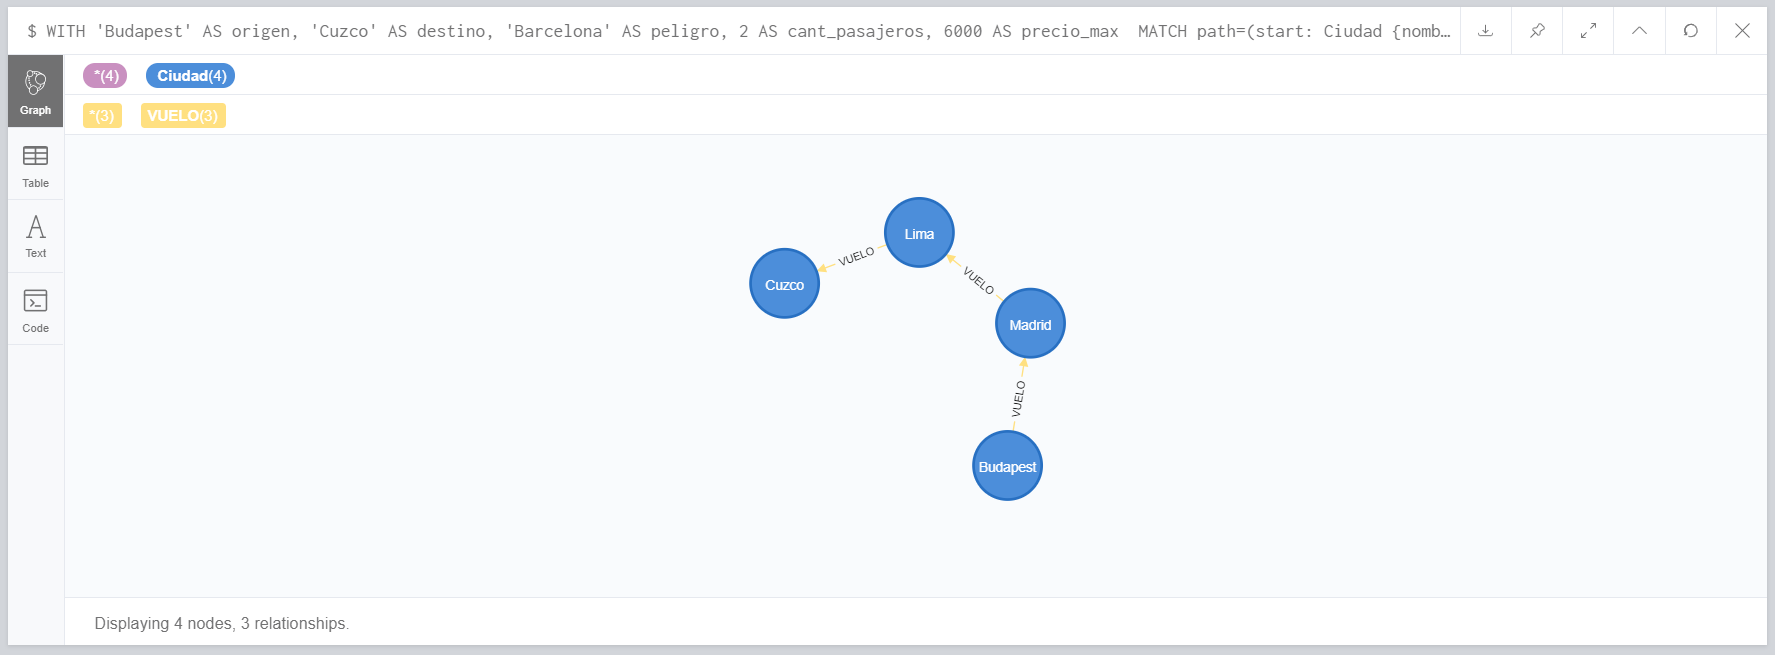
\includegraphics[scale=0.40]{./imagenes/consultaB-ejec4.png}
\end{center}
\end{document}

\newpage
\section*{Apendice X}



